\chapter{背景・目的}

\section{陣川町について}
陣川町は北海道函館市にあり(図\ref{map})、人口はおよそ3,300人の町である。
陣川町には「陣川あさひ町会」がある。
町会は陣川町の1,200世帯中約1,000世帯が加入している。
夏には参加者が約1,000人にもなる納涼まつりや
冬にはウィンターフェスティバルを行うなど積極的に活動している。
また、これらのイベント情報を多くの人に知らせる為に
町会役員がFacebookとLINE@を使い発信している。
しかし、積極的にイベントを開催する上で様々な問題を抱えている。
\\
\begin{figure}[h]
    \begin{center}
        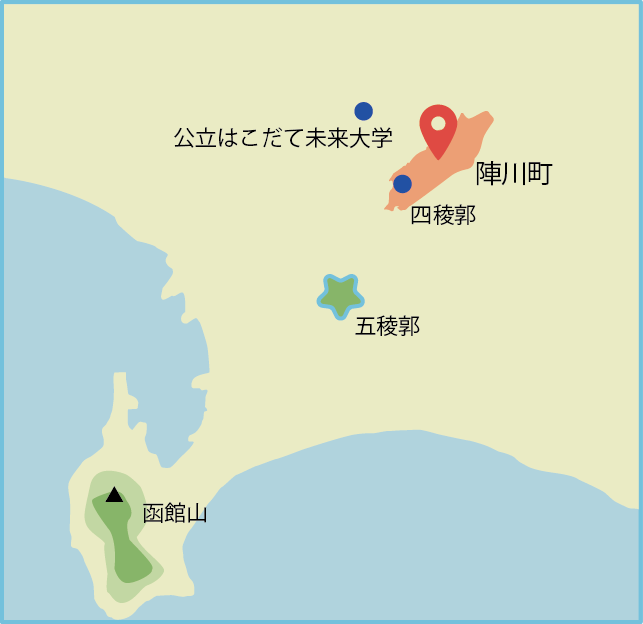
\includegraphics[keepaspectratio, scale=0.7]{map.png}
        \caption{陣川町周辺地図}
        \label{map}
    \end{center}
\end{figure}
\bunseki{船木綾香}

\section{町会が抱える問題}
\label{problems}
町会のイベントを開催する上での問題点は主に以下の6つである。
\begin{itemize}
    \item 情報内容に関する問題
    \begin{itemize}
        \item FacebookやLINE@ではイベントに関するお知らせはできるが、
              開催予定のイベントを一覧で見れない。
    \end{itemize}
    \item 情報伝達手段に関する問題
    \begin{itemize}
        \item イベントの情報をFacebookとLINE@に同一の内容を発信する手間がかかる。
        \item 町民のイベント申し込み方法が電話、FAX、メールの3つあり、イベント参加者の管理に手間がかかる。
        \item Facebookでは個人情報が漏れてしまうため参加申し込みができない。
        \item 役員だけで共有したい情報を町民に知られずに共有することがFacebookやLINE@ではできない。
    \end{itemize}
    \begin{itemize}
        \item イベント当日が悪天候の場合、参加者全員に対してイベントの中止、
              延期などの連絡を迅速に行うことができない。
    \end{itemize}
\end{itemize}
このように、町会はイベントを開催する上で様々な問題を抱えている。
\bunseki{船木綾香}

\section{目的}
本グループでは「陣川あさひ町会のイベント開催に関する問題を解決するサービスの提供をする」ことを目的とした。
\ref{problems}の通り、町会ではイベントを開催する上で様々な問題がある。
そこで本グループではそれらの問題を解決するアプリケーションを開発する。
\bunseki{船木綾香}
